\documentclass{llncs}
\usepackage{lipsum}

\usepackage{listings}
\usepackage{color}
\usepackage{setspace}

\usepackage{graphicx}

% \newcommand{\ts}{\textsuperscript}
% \usepackage{minted}

\definecolor{Code}{rgb}{0,0,0}
\definecolor{Decorators}{rgb}{0.5,0.5,0.5}
\definecolor{Numbers}{rgb}{0.5,0,0}
\definecolor{MatchingBrackets}{rgb}{0.25,0.5,0.5}
\definecolor{Keywords}{rgb}{0,0,1}
\definecolor{self}{rgb}{0,0,0}
\definecolor{Strings}{rgb}{0,0.63,0}
\definecolor{Comments}{rgb}{0,0.63,1}
\definecolor{Backquotes}{rgb}{0,0,0}
\definecolor{Classname}{rgb}{0,0,0}
\definecolor{FunctionName}{rgb}{0,0,0}
\definecolor{Operators}{rgb}{0,0,0}
\definecolor{Background}{rgb}{0.98,0.98,0.98}


\begin{document}
\title{MarketMaker:\\Multi-armed Bandits inspired trading algorithm}
\subtitle{Bristol Stock Exchange extension\\[1em]\today}
\author{Kacper \textbf{Sokol}---ks1591---45684}
\institute{Department of Computer Science,\\
  University of Bristol,\\
  Bristol, BS8 1UB\\
  \email{k.sokol.2011@my.bristol.ac.uk}}
%
\maketitle
%

\begin{abstract}
This paper introduces trading algorithm for \emph{Bristol Stock Exchange}%
\footnote{\url{https://github.com/davecliff/BristolStockExchange}} %
which is inspired by $k-$\texttt{lag} trend monitoring and \emph{Multi-armed Bandits} approach to \emph{exploration vs.\ exploitation} problem. Presented here algorithm is a wrapper for arbitrary Bristol Stock Exchange trading agent. It uses aforementioned models to determine the best possible time and type of order to issue and adjust its strategy to current trading session by adapting to opponents actions.
\end{abstract}
\keywords{Bristol, Stock, Exchange, $k-$\texttt{lag}, Multi-armed, Bandits, Market, Maker, Trading, Algorithm}

\section{Introduction}
Bristol Stock Exchange(BSE) is a simple and minimal simulation of \emph{limit order book}(LOB) financial exchange with single tradable security. In the market any trader can issue an order, where each new order replaces the old one. It also assumes zero latency in communication between the traders and the exchange and that information about newly issued orders is distributed among agents before the next order can be issued.\\

Designed algorithm trades on BSE using sub-traders---it is a wrapper for generic trading algorithm. In this study, used sub-traders are the one contained by default in BSE source code, but they can be easily changed. Each order is issued with sub-trader considered for given moment as the most profitable. The choice of which trader to use is governed by \emph{Upper Confidence Bound}(UCB) solution to \emph{Multi-armed Bandits}(MAB) problem.\\
Presented here trader differs from implemented in BSE agents as it is a \emph{Market-Maker}(MM): it trades with its own money and decides what and when to trade. On contrary, BSE own traders are \emph{sales traders} who receive external orders and make profit from the price difference they can make. Implemented MM tracks price trends with $k-$\texttt{lag} scheme to decide what order type and price it should issue.\\

To the best of my knowledge, presented here approach is first of its kind and has not been described or tested up to the present. The source code of the algorithm is available both in the \emph{\appendixname}, at the end of this paper (\emph{Listing~\ref{lst:MABmm}}), and on-line at: \url{https://github.com/So-Cool/MABtrader}.\\

\section{Methodology}
The stock exchange market is highly complex system, which dynamics is governed by supply and demand. Many different traders with wide range of strategies issue orders to trade securities with highest possible margin. The perfect agent should beat the competition by adapting to constantly changing market trends and structure. To address this issue I decided to use Multi-armed Bandits framework with \emph{Upper Confidence Bound} approach.\\

The decision when and what order to issue is based on two concepts: $k-$\texttt{lag} ($10-$\texttt{lag} in the experiment) of recent \emph{best} \emph{bids} and \emph{asks} on the LOB, and \emph{critical time point}. The first one identifies actual trend on the market to decide on the price and type of order to make. The latter detects approaching market closure---10\% of session time left in the experiment---to disable buying and short-selling (if allowed), and clear all possessed assets.\\
Chosen approach, does not require complex price analysis mechanism to maximise the trade profit as employed sub-traders work is to maximise their margin, which in this case flows to MM's pocket. Used sub-traders when given a price paid (received) for the asset will enforce it as minimal (maximal) and do their best to maximise profit.\\
The agent is capable of short-selling and has a predefined cap on number of possessed assets. For presented in this paper experiment it is allowed to collect up to $1$ asset, and short-selling is disabled.\\

To test designed \emph{MarketMaker} \textbf{22751} trading round were carried out each consisting of 33 traders: 16 buyers and 16 sellers of types Giveaway, Shaver, ZIC, and ZIP (consult BSE for details) with the ratio of the four types of traders being systematically varied across all possible non-zero values with 50 independent trials for each specification ratio. The one additional trader to this compilation is MAB MarketMaker.

\subsection{Order issuing}
Order issuing in presented trader is based on well known tool for time-series analysis called $k-$\texttt{lag}: in MM algorithm it calculates the difference between $k$\textsuperscript{th} most recent and current price at the market. It is used by the trader to calculate \emph{``best''} price trend of the LOB's \emph{bids} and \emph{asks}. As long as the corresponding trend in selected time window is rising (falling) the order is not issued. Once the trend has faltered the agent starts making offers: it buys assets based on minimum of recent ``best bids'' and its sell price, and sells assets based on maximum of ``best asks'' and its buy price.\\

The task of selecting trade margins is left to employed sub-traders. Each of them is sales trader and its task is to maximise margin of transaction based on given price. This allows the agent to issue orders with best of: paid price or current market price depending on which one is better. MM generates profit by utilising orders constructed by sub-trader and collecting achieved price margin.\\
Furthermore, for the experiment presented below the robot is only allowed to sell (or buy-back if previously short-sold) when it reaches its assets limit. If the cap is not reached the trader is allowed to decide whether to buy(-back) or (short-)sell based on speed of change in price trends.\\

The robot is capable of short-selling but due to BSE design this feature was disabled for the experiments. The main problem of short-selling is that once the trader issue a \emph{bid} or \emph{ask} order it has to continue issuing this particular type of order until it is crossed by other trader and realised. Otherwise, there is a possibility of crossing one's own offer or other robot's offer after changing one's own type of order. Hence, without substantial changes to BSE design interchangeably changing types of orders is not possible.\\

When the end of trading session is approaching, based on ``\texttt{panic}'' parameter the trader clears out all of its assets. If there exist short-sold items it will buy them back; if it holds any asset it will sell it; if it does not posses anything buying and selling is disabled.

\subsection{Sub-trader choosing with MAB}
The design of presented in this paper trader is inspired by gaining popularity in recent years framework for testing hypothesis: Multi-armed Bandits. MAB is rapidly replacing \emph{A-B testing} as it allows to dynamically change the environment it is running in with the best options for given moment and not only collect data for later analysis and decision making.\\
The main concept behind MAB is simply a row of slot machines each yielding some reward with unknown distribution. When an armed is pulled the machine generates reward which then can be used to better estimate its underlying distribution. The more often particular arm is played, the better user can understand its reward mechanism.\\
The main problem behind this setting is balancing the \emph{exploration} and \emph{exploitation} to achieve optimal cumulative long term reward. The \emph{exploration} of the environment in this simplistic scenario is playing under-discovered arms to learn more about their distributions, and \emph{exploitation} is playing the arm estimated to be the best according to current knowledge to quickly gain reward.\\
MAB is well documented challenge discussed in details by~\cite{berry+firstedt,gittins+glazebrook+weber}. Techniques solving posed by MAB problem are well known in on-line adversing world where they are used by companies such as Google~\cite{AYPSze12,ASMB:ASMB874}, LinkedIn~\cite{Tang:2013:AAF:2505515.2514700}, Microsoft~\cite{graepel2010web}, and Yahoo~\cite{Li:2010:CAP:1772690.1772758} to maximise the click-through rate by rearranging advertisements displayed on a web-page to be the best suited for given user.\\

To adopt MAB to MarketMaker trading algorithm I used the following analogies: the sub-traders are arms in the machine; the profit made by sub-trader on given order is the reward of an arm; and discovering profit associated with each sub-trader in current market is addressing exploration vs.\ exploitation problem.\\
I chose to solve this MAB trading problem with \emph{Upper Confidence Bound}(UCB)~\cite{white2012bandit} algorithm which is simple yet powerful technique to find optimal solution with least possible exploration. Furthermore, it prevents ``\emph{sticking}'' i.e.\ using arm (sub-trader) that is currently considered best but too little is known about other arms (sub-traders) to have strong evidence of its superiority.\\

Applying MAB algorithm in trading problem allows to probabilistic choose the best sub-trader based on current market structure. Furthermore, it does not require complex Bayesian statistics: collecting enormous amount of data in this scenario would be impractical. It also does not require to construct complex decision if-else model to react on changes taking place in the market structure. All these feature of chosen solution give MarketMaker great flexibility and adaptability potential.\\

The trader was designed to be a wrapper for trading algorithms compatible with BSE. It calls appropriate methods for each of its sub-traders to update their internal variables and issue them orders. Once a single trader is chosen for given round its order is collected and submitted to the exchange as MM's order.\\
The algorithm ensures that every sub-trader was tried at least once to collect the reward (profit on trade) information and be able to calculate its potential during the next order issuing process. By calculating UCB on rewards plus the uncertainty parameter of solution it chooses the best sub-trader for given situation. The uncertainty parameter ensures exploration of solutions considered for the moment as sub-optimal and acts as a changing lever if current sub-trader begins to under-perform in comparison with other available sub-traders until the reward is maximised.\\

In carried out experiments the opponents of MAB trader were the same as employed sub-traders. This situation places a strong assumption that MM knows the algorithms used by its competitors.

\section{Results}
% One / Multiple in the MArket # try LONGER SESSIONS to allow it to learn
To evaluate performance of designed trader I carried out described above experiment. Its basic statistic are available in \emph{Table~\ref{tab:stats}} presented below.\\

\begin{table}[ht]
  \centering
  \begin{tabular}{ p{5em} | p{5em}  p{5em}  p{5em} }
    name & mean & median & standard deviation \\
    \hline
    GWY  & $130.0$ &$ 130.0$ &$ 24.4$ \\
    MAB  & $12.7 $& $16.0 $& $37.9$ \\
    SHVR & $112.1$& $112.0 $& $13.2$\\
    ZIC  & $89.6 $& $87.0 $& $16.0$\\
    ZIP  & $130.3$ &$ 129.8$ & $12.2$
  \end{tabular}
  \vspace*{1em}
  \caption{Basic statistics for traders.\label{tab:stats}}
\end{table}

The visualisation of the above data is given in \emph{Figure~\ref{fig:box}} in form of a \emph{box-plot}.\\

\begin{figure}[ht]
  \centering
  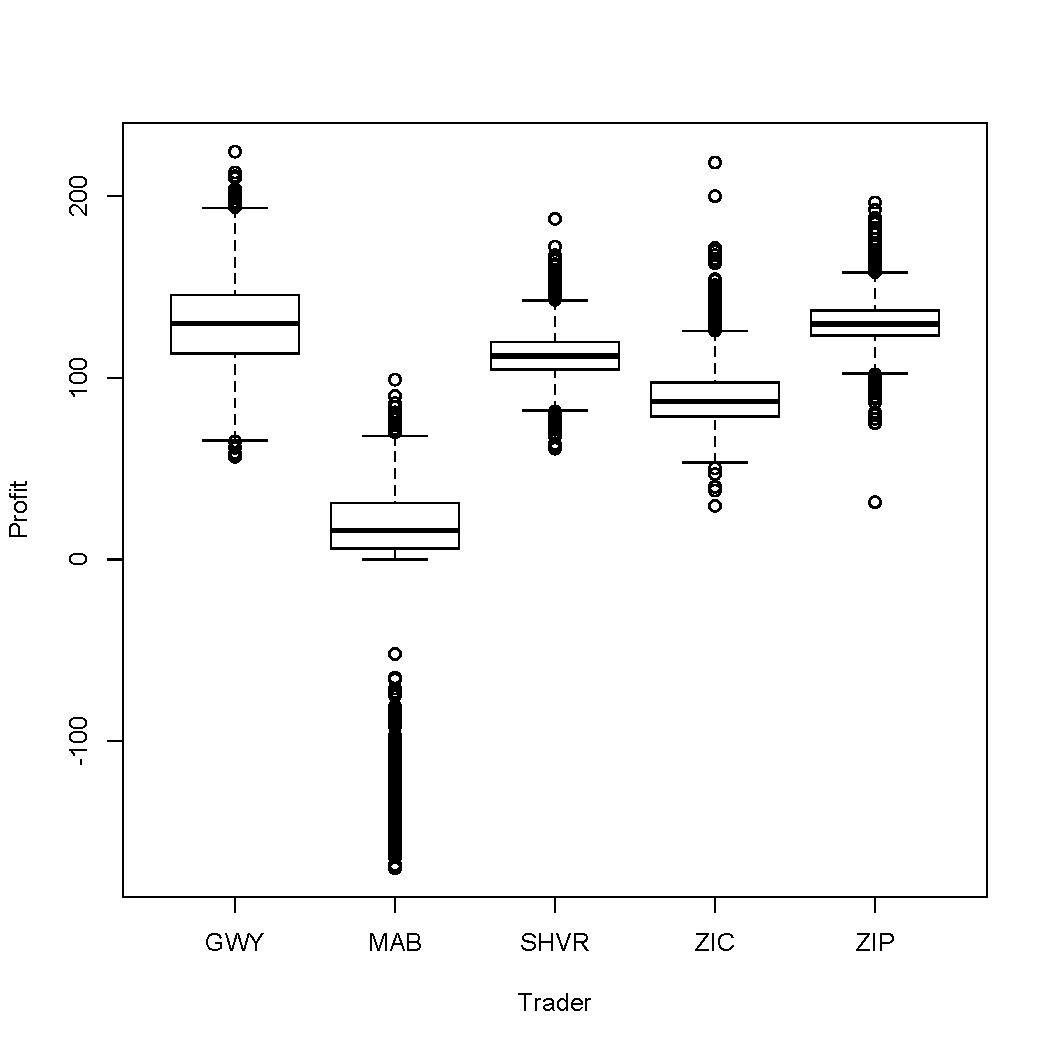
\includegraphics[width=.7\textwidth]{fig/box.pdf}
  \caption{Box-plot of profits for all traders.\label{fig:box}}
\end{figure}

The negative profit visible for MAB trader is possibly due to bought assets that were not sold before the end of a market session.\\
Basic inspection of these results yield conclusion that MAB MarketMaker is able to earn small amount of money in contrast to other algorithms trading at the BSE. To confirm this judgement I performed non-parametric \emph{Pairwise Wilcoxon-Mann-Whitney U Test} with 5\% significance level. Its results are available in \emph{Table~\ref{tab:wilcox}}.\\
Presented above box-plot has one more striking feature: it suggest that \texttt{GWY} and \texttt{ZIP} perform on average the same in the simulated environment.\\

\begin{table}[ht]
  \centering
  \begin{tabular}{ p{5em} | p{5em} p{5em} p{5em} p{5em} }
         &GWY    &MAB    &SHVR   &ZIC   \\
    \hline
    MAB  &$<2e-16 $&$-      $&$-      $&$-     $\\
    SHVR &$<2e-16 $&$<2e-16 $&$-      $&$-     $\\
    ZIC  &$<2e-16 $&$<2e-16 $&$<2e-16 $&$-     $\\
    ZIP  &$0.28   $&$<2e-16 $&$<2e-16 $&$<2e-16$
  \end{tabular}
  \vspace*{1em}
  \caption{Results of Pairwise Wilcoxon-Mann-Whitney U Test.\label{tab:wilcox}}
\end{table}

Above results confirm that MAB performs significantly worse than all other algorithms: $p-$value is significantly smaller than significance level. Furthermore $p-$value for the \texttt{GWY}-\texttt{ZIP} pair confirms our observation that profits of both algorithm are statistically indistinguishable: $0.28$ $p-$value is larger than fixed $0.05$ significance level. The test suggests the following traders order---best to worst:\\
$$
\mathtt{GWY} = \mathtt{ZIP} > \mathtt{SHVR} > \mathtt{ZIC} > \mathtt{MAB}
$$

\begin{figure}[ht]
  \centering
  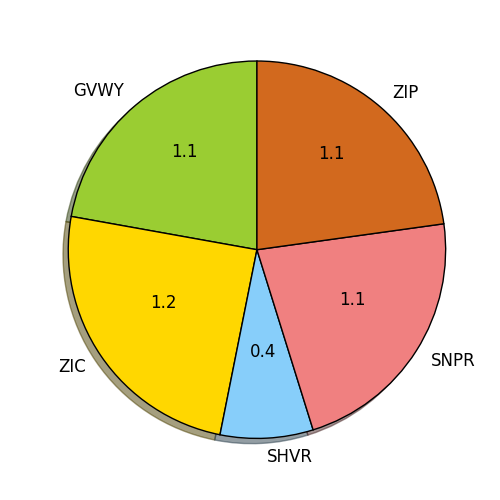
\includegraphics[width=.5\textwidth]{fig/pie.png}
  \caption{Sub-traders used by MAB MarketMaker.\label{fig:MABalgo}}
\end{figure}

Finally, \emph{Figure~\ref{fig:MABalgo}} above, indicates the average number of times that each sub-trader was used during single trading session. Based on collected data, the average number of trades made by MAB per market session is \textbf{4.78}.\\



\section{Discussion}
Presented in this paper solution is based on well known price trend analysis and relatively novel probabilistic approach to trading agents inspired by Multi-armed Bandits. As stock exchange markets contains vast number of independent and self-centred agents hence it is important to ensure that produced trader can quickly adapt to the environment it is placed in.\\
The key strength of my solution is simple yet effective price change detection mechanism and modularity of used sub-traders. It is possible to use relatively large number of them, each adapted to different market structure. Without explicitly specifying rules governing use of particular sub-trader, UCB will try each solution and based on collected profit it will converge to most profitable one. In case of sudden market shift the algorithm will automatically re-explore sub-traders' profit to check for possible improvements of current strategy.\\

Based on presented above statistical analysis MAB MarketMaker performs relatively poor in comparison with all other algorithms used in experiment: it earns on average 77 units less than second worst trader. It detects only a few possibilities to earn money---\textbf{4.75} trades per session. This relatively low average number of trades per sessions undermines the concept of using Multi-armed Bandits as a mechanism for choosing sub-trader. Almost uniform sub-traders engagement (\emph{Figure~\ref{fig:MABalgo}}) indicates that full potential of MAB is not used as the algorithm did not have enough opportunity to converge to the best solution.


\section{Conclusion}
Presented here approach to MarketMaker traders uses 
Used approach is novel and the paper presents only rough framework how to use it. There is still lot of work to be done and research to be carried out to understand use of Multi-armed Bandits in trading algorithms.\\

The longer sessions and more trading opportunities is needed to allow MAB algorithm to learn and use the best strategy for current market structure.\\

Inspect why ZIP and GVY perform similary.\\

This study engages only use of predefined in BSE traders. Presented here framework can be easily generalised to use more complex and diversified sub-traders covering wider range of possible market situations. The next viable goal extending this study would be to employ more sub-traders and check the performance of proposed solution.\\
Furthermore, another study is needed to check the behaviour of trader when it can change its status from selling to buying without making a transaction. Enabling multiple orders and short-selling might also be worth inspecting. Also interesting should be deploying multiple MAB MArketMakers and see how they interact.\\
Also another study is needed inspecting behaviour of MAB trader where used sub-traders differ from other strategies used by other agents in the market.\\
Finally, as MAB strategies show their full potential in long run experiments another study should be carried out with longer trading sessions.


\vfill
\bibliographystyle{plain}
\bibliography{ref}

\newpage
% \begin{appendices}
\section*{\appendixname: MAB MarketMaker source code\label{app:MABmm}}

% \inputminted[
% frame=lines,
% framesep=2mm,
% baselinestretch=1.2,
% fontsize=\footnotesize,
% linenos
% ]{python}{../code/marketMaker.py}

\lstset{
captionpos=b,
breaklines=true,
caption=MAB MarketMaker source code,
label=lst:MABmm,
%
numbers=left,
numberstyle=\footnotesize,
numbersep=1em,
xleftmargin=1em,
framextopmargin=2em,
framexbottommargin=2em,
showspaces=false,
showtabs=false,
showstringspaces=false,
frame=l,
tabsize=4,
% Basic
basicstyle=\ttfamily\small\setstretch{1},
backgroundcolor=\color{Background},
language=Python,
% Comments
commentstyle=\color{Comments}\slshape,
% Strings
stringstyle=\color{Strings},
morecomment=[s][\color{Strings}]{"""}{"""},
morecomment=[s][\color{Strings}]{'''}{'''},
% keywords
morekeywords={import,from,class,def,for,while,if,is,in,elif,else,not,and,or,print,break,continue,return,True,False,None,access,as,,del,except,exec,finally,global,import,lambda,pass,print,raise,try,assert},
keywordstyle={\color{Keywords}\bfseries},
% additional keywords
morekeywords={[2]@invariant},
keywordstyle={[2]\color{Decorators}\slshape},
emph={self},
emphstyle={\color{self}\slshape},
% 
}\lstinputlisting{../code/marketMaker.py}


\end{document}
